\documentclass[conference]{IEEEtran}
\usepackage[T1]{fontenc}
\usepackage{amsmath,amssymb,booktabs,graphicx,url,array}
\usepackage[hidelinks]{hyperref}
\newcommand{\Prb}{\mathbb{P}}
\newcommand{\E}{\mathbb{E}}
\newcommand{\ind}{\mathbf{1}}
\title{Position: PII Redaction Claims Must\protect\\Specify the Release Mechanism}
\author{\IEEEauthorblockN{Anonymous Author}}
\begin{document}
\maketitle
\begin{abstract}
An updated personally identifiable information (PII) redaction system should inherit a numerical release claim only through a preservation argument, a valid transfer calculation, or new evidence. This paper applies established assurance-maintenance principles to the protection policy, failure event, release mechanism, and population underlying that claim. It argues for retaining output validity before normalization, reporting applicability and release counts jointly, and attaching evidence to the evaluated loss and recipient-visible channels. Conditional failure among released records and unconditional failed-release probability support different decisions. Exact constructions distinguish changes in protection from changes in the evaluated denominator. An analysis of published LeakageBench aggregates derives feasible matching-failure ranges after invalid outputs are withheld and identifies the information needed for an exact recount. A parameterized workflow then carries a hypothetical audit through two updates: mask expansion preserves its containment bound, while a stricter gate leaves the original target unsupported because fewer relevant observations remain. Established selective-risk methods supply the statistical machinery. A completed reuse record assigns responsibilities, specifies conditions for continued use, and shows when another audit can be avoided. The contribution concerns redaction-specific evidence requirements, with annotated removal kept distinct from adversarial inference.
\end{abstract}
\begin{IEEEkeywords}
PII redaction, privacy evaluation, selective prediction, risk control
\end{IEEEkeywords}

\section{Introduction}
A numerical redaction claim is often used to justify sending information outside a protected environment. That decision depends on a complete mechanism: parsing an input, identifying protected content, producing an output, and deciding whether to release it. A model score describes only part of this process. Even a valid bound on an end-to-end failure rate can lose its meaning when a release rule, protection policy, or output format changes.

\textbf{An updated redaction system should inherit a numerical release claim only through an applicable preservation argument, a valid transfer calculation, or new evidence.} The claim must identify its mechanism, loss, denominator, and population so that this justification can be assessed. This requirement concerns claims used to support release decisions; it does not require every diagnostic benchmark to certify deployment safety.

The position has three concrete reporting consequences. First, retain output validity before normalization: converting a failure to an empty prediction can erase the distinction needed to evaluate a later release gate. Second, report policy applicability and release decisions jointly with the evaluated failures; separate marginal rates can leave the post-update denominator unresolved. Third, attach each reused result to its loss and delivered channels: expanding an opaque mask can preserve concealment while worsening geometric matching, and an added text layer can invalidate a claim about the complete output. These requirements determine whether existing evidence supports a recount, a preservation argument, or reassessment.

Consider a constructed population of 1,000 equally likely inputs. A system releases 800 records, eight of which violate its removal policy. Its conditional failure rate is 1\%. A stricter gate releases 80 of those records, retaining the same eight failures. Conditional failure becomes 10\%, although no retained output changed and the unconditional probability of a failed release remains 0.8\%. Restriction preserves one quantity but invalidates an earlier statement about another. This example establishes a possible failure of evidence reuse, not its prevalence in operating systems.

The reverse denominator effect also matters. Releasing additional records containing no protected information can lower conditional failure while leaving protection of sensitive records unchanged. Thus, the position cannot be reduced to replacing entity scores with a preferred document-level fraction. The denominator itself expresses an operational question. Both conditional failure among released records and unconditional failed-release probability can be appropriate, provided their interpretation is explicit.

The need to evaluate privacy beyond entity recognition is established. Lison et al. advocate disclosure-risk-aware anonymization~\cite{lison2021}; TAB, RedactionBench, LeakageBench, and subject-level inference assessment develop richer evaluation targets~\cite{tab2022,redactionbench2026,leakagebench2026,spia2026}. Policy-conditioned security and utility are also addressed by RedacBench~\cite{redacbench2026}. Selective prediction and Learn then Test (LTT) supply methods for controlling losses on accepted outputs~\cite{elyaniv2010,geifman2017,angelopoulos2025}. The question developed here is how evidence from these evaluations should be interpreted when the redaction mechanism changes.

The evidence consists of analytical constructions, a source-based protocol analysis, and deterministic numerical calculations. In the published-aggregate application, withholding invalid outputs alone cannot reduce critical matching failure below 98\% for the five systems with nonunit validity under the stated assumptions. The application also identifies the joint counts needed for an exact recount. No new model-performance measurements or evidence of widespread misuse are claimed. The proposed record makes the resulting update decisions inspectable and permits reuse where a structural argument justifies it.

\section{Related Work}
\subsection{Privacy targets and utility}
The methodological case for moving beyond sequence labeling predates this paper~\cite{lison2021}. TAB incorporates privacy-oriented annotations, including identifier types and coreference~\cite{tab2022}. RedactionBench evaluates contextual redaction with character-based treatment of alternative boundaries~\cite{redactionbench2026}. RedacBench, a separate benchmark, evaluates policy-conditioned removal and preservation of information using proposition annotations~\cite{redacbench2026}. Tau-Eval makes utility dependent on the intended downstream task~\cite{taueval2025}. These studies already establish that the protection policy and useful information retained belong in an evaluation.

LeakageBench evaluates omissions at the page level in document images and distinguishes supported-schema from full-schema performance~\cite{leakagebench2026}. Its explicit challenge-set scope makes it a useful case for examining which additional assumptions a deployment claim would need. SPIA and work on inference with language models address information about people that remains recoverable after transformation~\cite{spia2026,staab2024}. Removal of annotated content is therefore only one possible loss. A statistical removal bound is also distinct from differential privacy, which constrains a mechanism under a neighboring-dataset relation~\cite{dwork2014}.

\subsection{Risk control and the proposed addition}
Selective prediction formalizes the relation between conditional error and coverage~\cite{elyaniv2010,geifman2017}. Risk-controlling prediction sets provide finite-sample control of a chosen loss~\cite{bates2021}. LTT includes accepted-sample binomial calibration, structured outputs, multiple risks, and selection among operating points~\cite{angelopoulos2025}. The confidence calculations used here are applications of that established framework and the Clopper--Pearson bound~\cite{clopper1934}. Conformal risk control supplies a different, marginal expected-loss guarantee under its stated assumptions~\cite{angelopoulos2024}; its name alone does not establish conditional protection under an arbitrary downstream gate.

Maintaining assurance after system changes is established prior work. Transfer assurance identifies which parts of an ML assurance case remain applicable and which require reassessment~\cite{picardi2023}; change-impact analysis links modified artifacts to affected claims and recommended updates~\cite{carlan2022}. Certified model-update methods also provide preservation arguments through invariant parameter domains~\cite{elmecker2026}. The present position applies these principles to redaction losses, denominators, and observable channels. Its contribution is to distinguish updates that preserve containment from those that change acceptance, evaluation eligibility, or protected information, and to specify the evidence needed for the corresponding release claim. The protocol application in Section~\ref{sec:case} and practical record in Section~\ref{sec:practice} develop that narrower contribution.

\section{Specify the Claim and Its Denominator}
\subsection{Protection, observation, and release}
Let $X\sim P$ be an input unit. Depending on the disclosure, a unit may be a document, a conversation, or the combined records about a person. A policy $\pi$ identifies protected subjects and content in the intended recipient context. A pipeline $h$ produces the recipient-visible object $Y_h(X)$, and a gate $g_h(X)\in\{0,1\}$ determines release. The pipeline includes parsing, OCR if used, candidate generation, prompts, thresholds, chunk aggregation, rendering, and fallback behavior. Probabilities include any independent per-unit pipeline randomness used by the audited mechanism.

For a deletion-only task, let $S_\pi(x)$ be the required source positions and $R_h(x)$ the positions actually concealed in the released representation. A complete-removal failure is
\begin{equation}
 L_{\pi,h}(x)=\ind\{S_\pi(x)\not\subseteq R_h(x)\}.
 \label{eq:span}
\end{equation}
Overlapping regions are interpreted through their union. Partial-disclosure policies need another loss. Source containment is meaningful only for compatible source and output representations; generative rewriting requires its own correspondence or semantic evaluation.

The observation must include every supplied channel. Concealing pixels does not conceal searchable text carried in the same file. A release or withholding decision visible to the recipient may itself disclose information; the containment loss does not assess that channel. An attack-success loss can instead evaluate a specified attacker, auxiliary information, query budget, and target. Its bound applies to that attack under the audited conditions, not to all possible attackers. Neither precise confidence intervals nor extensive masking repair an incorrectly specified loss.

\subsection{Three related quantities}
Suppressing subscripts, define coverage, conditional risk, and joint failed-release probability by
\begin{align}
 c&=\Prb(g=1), & r&=\Prb(L=1\mid g=1),\label{eq:risk}\\
 j&=\Prb(g=1,L=1)=cr.&&\label{eq:joint}
\end{align}
Conditional risk requires $c>0$. Withholding everything gives $j=0$ and zero coverage, not a defined zero value of $r$. A limit on failures per incoming unit concerns $j$; a quality requirement on released records concerns $r$. Reporting both reveals whether a change reduces failures, changes release volume, or redistributes failures among outputs.

Protected-content prevalence is needed to interpret $r$ for the span loss. Let $Z=\ind\{S_\pi(X)\ne\varnothing\}$, using policy annotations rather than predicted entities, and define
\begin{equation}
 p_+=\Prb(Z=1\mid g=1),\qquad
 r_+=\Prb(L=1\mid g=1,Z=1).
\end{equation}
For $p_+>0$, the fact that $L=0$ when $Z=0$ gives
\begin{equation}
 r=p_+r_+.
 \label{eq:prevalence}
\end{equation}
If $p_+=0$, then $r=0$ and $r_+$ is undefined. For example, 100 sensitive records with ten failures have $r_+=10\%$. Releasing another 900 records with no protected content reduces $r$ from 10\% to 1\%, while $r_+$ remains 10\%. This is a valid change in aggregate risk, but does not establish better protection of sensitive records. Figure~\ref{fig:changes} contrasts it with gate restriction. Changes in $p_+$ and $r_+$ should therefore be reported separately when protection of sensitive records motivates the claim.

\subsection{Population and annotation scope}
A challenge set can expose vulnerabilities without estimating their frequency in deployment. A population claim requires a sampling argument, including source and evaluation period. Multiple pages from one document, or records from one person, are not automatically independent units. The release unit and the sampling unit must support the promised level of protection; independent-looking fragments do not create a person-level guarantee.

A policy and annotation protocol should be fixed before the final audit. Relabeling failed items as out of scope changes the question. Candidate-only annotation is especially problematic: omitted regions are missing from both the predictions and the reference. For a candidate-restricted masker without a fallback, any required position outside every candidate is necessarily missed. The resulting failure floor is a property of the complete mechanism and cannot be eliminated by adjusting its classifier threshold. Labels must therefore cover the declared policy independently of the candidate list.

\section{When Evidence Survives a Change}
\subsection{Aggregation is necessary but insufficient}
Mention recall does not determine complete-record failure. Among 1,000 records with 100 protected mentions each, 1,000 misses can be concentrated in ten records or spread across every record. Both systems have 99\% recall, but failed-record proportions are 1\% and 100\%. The artifact gives the general counting bounds. Aggregation at the release unit is necessary, while concentration of harm, the denominator, and conditions for evidence reuse still require separate assessment.

\subsection{Preservation by pointwise improvement}
For an unchanged population and identical acceptance decisions almost surely, $L'\leq L$ on released units implies $r'\leq r$ and $j'\leq j$. A valid upper bound therefore transfers. For Eq.~\eqref{eq:span}, expanding concealed positions pointwise with the same policy is sufficient. Requiring only a subset of previously protected positions also decreases this loss, but weakens the promise rather than demonstrating improved protection under the old policy.

Identical gate code is insufficient if its inputs or scores changed. Likewise, a lower detection threshold is monotone only if overlap resolution, rendering, and other processing retain every earlier mask. A finite set of successful regression checks does not prove an almost-sure property. Evidence for preservation can instead follow from the implementation, for example explicitly taking the union of old and additional masks while fixing acceptance decisions. For randomized mechanisms, nesting must hold almost surely under a specified coupling with the correct marginal distributions.

These arguments concern a specified loss. Mask expansion does not necessarily reduce the success of a fixed attacker, and newly chosen mask locations may expose information. An information-theoretic argument would require the complete new observation to be a postprocessing of the old observation and a compatible target and population. Containment alone supplies neither condition.

\subsection{Restricted release and a useful diagnostic}
Suppose $g'\leq g$ and $L'\leq L$ on retained units. For $0<c'\leq c$,
\begin{equation}
 r'=\frac{\E[g'L']}{c'}\leq\frac{c}{c'}r,
 \qquad j'\leq j.
 \label{eq:transfer}
\end{equation}
The first bound is capped at one. Without changing the loss, retaining all failures attains the uncapped bound when feasible; retaining only failures attains the cap when enough failures are available. Thus, a bound $r\leq\alpha$ generally transfers only as $r'\leq\min(1,\alpha c/c')$. Coverage estimates cannot be substituted as exact population quantities; Section~\ref{sec:transferaudit} accounts for their uncertainty.

For unchanged outputs, the cause of any conditional-risk increase can be located directly. Put $\rho=c'/c$, $r_{\rm keep}=\Prb(L=1\mid g'=1)$, and $r_{\rm drop}=\Prb(L=1\mid g=1,g'=0)$. When $0<\rho<1$,
\begin{align}
 r&=\rho r_{\rm keep}+(1-\rho)r_{\rm drop},\label{eq:mixture}\\
 r'-r&=(1-\rho)(r_{\rm keep}-r_{\rm drop}).\label{eq:diagnostic}
\end{align}
Conditional risk rises exactly when the gate discards a lower-risk stratum. If masks also change, subtract $\Delta_{\rm keep}=\E[L-L'\mid g'=1]$ from the right side of Eq.~\eqref{eq:diagnostic}. This separates selection from changes to retained outputs. At $\rho=1$ the selection term vanishes, without requiring a defined discarded-stratum risk.

These identities suggest a paired evaluation: record the old loss on retained and discarded units, then evaluate any new loss on retained units. An aggregate before/after score conceals that distinction. In the opening construction, $\rho=0.1$, $r_{\rm keep}=0.1$, and $r_{\rm drop}=0$, which explains the increase without assigning any deterioration to the redactor.

\subsection{When threshold tightening is justified}
The possibility of harmful selection does not mean every stricter gate needs to increase risk. Fix a transformation, a document score $T$, and gates $g_t=\ind\{T\leq t\}$. If $\eta(s)=\E[L\mid T=s]$ is nondecreasing almost surely, lowering $t$ cannot increase conditional risk at positive coverage. The retained score range has no higher mean failure than the discarded range, so Eq.~\eqref{eq:mixture} establishes the result. Exact calibration $\eta(s)=s$ is sufficient; calibration of individual mention confidences is not this document-level condition.

Calibration on its own also does not protect arbitrary subsequent selection. A constant document score of 1\% is calibrated in a population where a group of mass 10\% has 10\% failure and the remainder has none. A gate retaining that group has 10\% failure. The distinction is between tightening the same appropriately ordered score and selecting on another feature. This gives the central warning a boundary: preservation follows from a demonstrated relationship between the gate and the stated loss, not from the word ``stricter.''

\begin{figure*}[t]
 \centering
 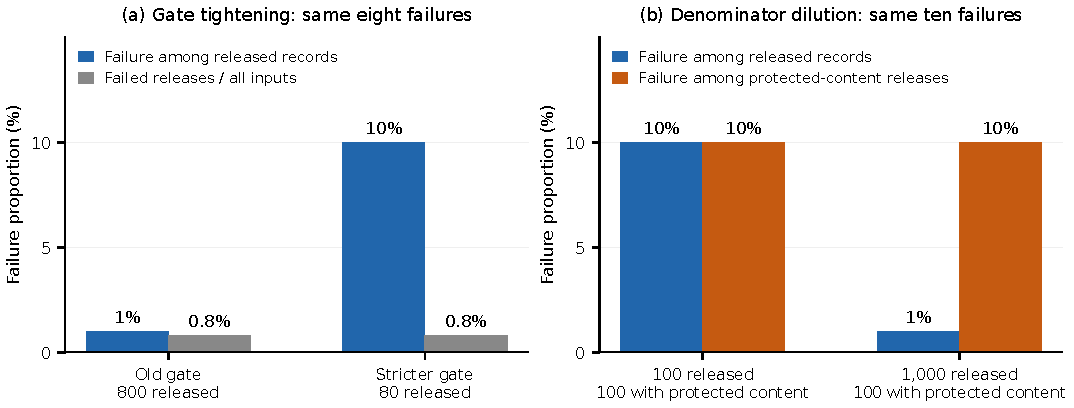
\includegraphics[width=\textwidth]{figures/release_changes.pdf}
 \caption{Exact hypothetical populations illustrate two denominator effects. A stricter gate can retain a higher-risk subset, while accepting records without protected content can lower aggregate conditional risk without improving protection of sensitive records. Neither panel reports model measurements.}
 \label{fig:changes}
\end{figure*}

\section{A Published Protocol and Its Conditions of Reuse}
\label{sec:case}
\subsection{What the published evaluation measures}
LeakageBench v1 provides a concrete protocol case~\cite{leakagebench2026}. It evaluates pages independently. DocLeak counts pages with any unmatched in-scope annotation among pages containing at least one in-scope gold annotation, whether matched or unmatched. The headline matching rule is greedy, one-to-one, type-aware, and uses intersection-over-union (IoU) of at least 0.75~\cite[Secs.~3.1, 3.3--3.4]{leakagebench2026}. The 500 pages derive from 291 documents~\cite[Table~2]{leakagebench2026}. Full-schema scoring counts unsupported types as misses; supported-schema scoring filters the gold types. Unusable outputs become empty predictions~\cite[Secs.~5.1, 6]{leakagebench2026}. The paper explicitly limits its data to a challenge set and distinguishes IoU from direct concealment~\cite[Sec.~4.1, Limitations]{leakagebench2026}. These choices support a scoped diagnostic evaluation.

This protocol exposes three distinct predicates: a page contains in-scope content, its predictions meet the matching rule, and an operator releases its output. DocLeak's eligibility condition corresponds to $Z$, whereas a release policy defines $g$. Equation~\eqref{eq:prevalence} explains why a score on applicable pages cannot directly supply a failure rate among all released pages. Filtering the gold schema may change both the failure event and the applicable-page denominator. A smaller supported-schema score therefore does not, by itself, demonstrate improved protection under the original policy.

\subsection{A realistic release modification}
Consider a hypothetical operator that starts from release-all and accepts exactly the outputs that pass a fixed parsing and validation procedure. Define $V=1$ when that procedure yields a usable prediction list, recording the flag before unusable outputs are replaced by empty predictions. A valid empty list may have $V=1$; a parsing or validation failure normalized to the same list has $V=0$. Set the new release gate to $g'=V$, with no additional filter. This rule is a hypothetical application of the published scoring convention, not a reported deployment.

Let $L_{\rm match}$ denote matching failure. On an applicable page, $V=0$ produces empty predictions, so $V=0,Z=1$ implies $L_{\rm match}=1$. Removing those pages cannot worsen matching failure on that subset. If $d$ is the original applicable-page failure fraction and $v_+$ the fraction of applicable pages with $V=1$, the matching-failure fraction among retained applicable pages is
\begin{equation}
 d_{\rm valid}=\frac{d-(1-v_+)}{v_+}\leq d,\qquad v_+>0.
\end{equation}
This preservation follows from the scoring rule. It does not automatically cover complete concealment or failure among all released pages. Overall validity need not equal $v_+$; a change in protected-content prevalence can alter the all-release rate. Validity, applicability, loss, and release should therefore be recorded jointly.

An exact recount can use sufficient joint counts. Reconstructing it from individual outputs requires labels and either raw model outputs or normalized predictions together with retained validity flags. Normalized prediction lists alone may not distinguish successful empty predictions from failures. Recounting fixed outputs needs no new model execution, but does not make a challenge set representative of deployment. If whole documents are released, their pages must first be grouped and the document loss defined; repeated pages are not independent document-level observations.

Changing the model's requested entity list is a different modification: the predictions themselves can change, so retaining the old outputs is insufficient. Releasing a searchable PDF instead of only an image changes the observable channels. These examples lead to distinct actions, respectively recounting a fixed evaluation, reevaluating predictions under the policy, and auditing the complete output representation. A single claim that a system is ``based on the evaluated model'' cannot distinguish them.

\subsection{What the reported aggregates support after withholding}
\label{sec:publicapplication}
The validity gate can be applied analytically to published results without inventing per-page predictions. Table~3 of LeakageBench v1 reports critical DocLeak and validity for 14 systems on 500 pages~\cite[Sec.~6, Table~3]{leakagebench2026}. For this application, $V$ is the published page-validity indicator, with $V=0$ identifying unusable outputs scored as empty predictions. The calculation requires this correspondence; rejecting individual boxes while retaining usable predictions is a different event. Applicability means at least one Direct or Linkage annotation, and failure uses the published typed IoU matching rule. The full-schema rows share this applicability set; the model-dependent filtering in Table~4 is not used.

Let $D$ be the number of applicable pages, $F_i$ their failures for system $i$, $B_i$ its invalid outputs among all 500 pages, and $A_i$ the invalid outputs on applicable pages. The published convention makes those $A_i$ pages failures. Feasible integer counts satisfy
\begin{equation}
 \max(0,B_i-(500-D))\leq A_i\leq\min(B_i,F_i),
\end{equation}
and give $d_{{\rm valid},i}=(F_i-A_i)/(D-A_i)$ when $D>A_i$. Let $\widehat d_i$ and $\widehat v_i$ be the reported critical failure and validity fractions. Nearest rounding to three decimals imposes
\begin{equation}
 \left|\frac{F_i}{D}-\widehat d_i\right|\leq0.0005,
 \qquad
 \left|\frac{500-B_i}{500}-\widehat v_i\right|\leq0.0005.
 \label{eq:rounding}
\end{equation}
All counts are integers, with $1\leq D\leq500$, $0\leq F_i\leq D$, and $0\leq B_i\leq500$. Including both endpoints admits either rounding tie convention. Intersecting the feasible counts for all 14 systems at a common $D$ restricts $D$ to 493--500; each $B_i$ is uniquely determined. The artifact enumerates these compatible configurations without asserting which occurred.

\begin{table}[t]
\centering
\caption{Derived extrema after withholding invalid outputs, using the Table~3 marginals and stated rounding assumptions. All five systems with reported validity below one are shown. Rates concern critical matching failure among retained applicable pages; endpoints are approximate percentages.}
\label{tab:aggregate}
\small
\begin{tabular}{@{}p{0.37\columnwidth}rp{0.35\columnwidth}@{}}
\toprule
System & Valid pages & Failure range (\%) \\
\midrule
Presidio & 498 & 98.9817--98.9960 \\
GLiNER2 & 499 & 99.3902--99.3988 \\
OpenAI Privacy Filter & 403 & 98.7374--98.7593 \\
Qwen3-VL-32B & 333 & 99.6933--99.6997 \\
InternVL3-38B & 270 & 100 \\
\bottomrule
\end{tabular}
\end{table}

Table~\ref{tab:aggregate} establishes a bounded consequence for this proposed gate: even after withholding invalid outputs, critical matching failure remains above 98\% for each system with nonunit validity under these assumptions. Thus, validity-only withholding cannot meet a matching-failure target below 98\% for these systems on this challenge set. The result tests an additional release rule applied to the benchmark's scoped diagnostic evaluation. The intervals are feasible-count ranges, not confidence intervals, deployment risks, or measures of complete concealment.

For a worked row, OpenAI Privacy Filter reports $\widehat d=0.990$ and $\widehat v=0.806$, so $B=97$. At the compatible value $D=493$, Eq.~\eqref{eq:rounding} gives $487.8235\leq F\leq488.3165$, hence $F=488$. The intersection constraint allows $90\leq A\leq97$. Its endpoints give $(488-97)/(493-97)=391/396$ and $(488-90)/(493-90)=398/403$. These are compatible completions, not observed page-level outcomes. Publishing $D$ and $A$, together with the failure count or a rate precise enough to determine it, permits an exact recount for this gate. Once $D$ is known, the reported three-decimal rate determines $F$ uniquely at these denominators.

The reporting assumptions have inspectable consequences. Using only the Privacy Filter row permits a range from 0 to about 99.05\%; the other rows constrain the shared denominator and make the stronger conclusion possible. Truncation instead of nearest rounding leaves only $D=500$ compatible with all 14 rows and preserves the above-98\% conclusion. No model was executed, and no claim is made about an operator having deployed this gate.

\subsection{Why the loss matters for mask expansion}
A geometric construction makes the difference between matching and concealment explicit. Let the entire gold rectangle be the policy-required region, with area $a$, and suppose a predicted opaque mask equals it. Its IoU is one and its containment loss is zero. Expand the mask to a containing rectangle of area $2a$, with the same type. IoU falls to $1/2$, below 0.75, although every sensitive pixel remains concealed. Conversely, an opaque prediction entirely inside the gold rectangle and covering 80\% of its area passes the IoU threshold while leaving 20\% uncovered.

These constructed geometries do not describe measured benchmark outputs. They establish that an IoU-matching loss cannot be substituted for complete concealment when applying the preservation argument. For an image release, that argument requires evaluating the union of actually rendered masks against the required regions, with other delivered channels considered separately. The practical consequence is specific: a mask-expansion update may preserve a containment claim while worsening a matching score, and a passing match need not establish complete removal. The appropriate response is to name and evaluate both losses where both matter.

\section{Evidence for a Specified Claim}
\subsection{Fix the audit design before observing outcomes}
Fix the mechanism, policy, loss, and gate independently of the final audit, and choose the number $N$ of incoming units in advance. Draw $N$ independent, identically distributed units from $P$ and apply independent per-unit randomness if used. Conditional on $n>0$ releases, their failure count $k$ is binomial with parameter $r$, assuming the labels correctly evaluate the specified loss. A one-sided Clopper--Pearson upper bound~\cite{clopper1934} is
\begin{equation}
 U(k,n;\delta)=
 \begin{cases}
 \operatorname{Beta}^{-1}(1-\delta;k+1,n-k),&k<n,\\
 1,&k=n.
 \end{cases}
 \label{eq:cp}
\end{equation}
If $n=0$, report conditional risk as not estimable and use the uninformative bound one. Direct sampling from a specified released population is another valid design, provided its sample size is fixed independently of failures. Outcome-dependent stopping needs an appropriate sequential procedure.

The same construction targets $j$ using $k$ failed releases among $N$ inputs. For $r_+$, it uses failures among released units independently annotated as containing protected content. These are different counts for different claims. Their overlapping observations do not create additional independent units. Separately estimated claims require a valid simultaneous procedure when joint coverage is intended. For $H$ prespecified claims, a simple allocation is $\delta/H$ per claim; independence between claims is unnecessary. Selecting a mechanism on the audit generally requires selection-aware methods such as LTT~\cite{angelopoulos2025} or new independent evidence.

Structural inheritance is different. If every permitted update has the same gate, policy, and population and satisfies $L_u\leq L_0$ pointwise, the single event $r_0\leq U$ implies $r_u\leq U$ for every such update. No additional confidence allocation is needed for these inherited bounds. The update may even be selected after the audit if the relation holds for every possible selected update. Empirically observing dominance on the audit is insufficient for this argument.

With zero failures, $U(0,n;\delta)=1-\delta^{1/n}$. At 95\% confidence, 500 independent releases give approximately 0.597\%, while a 0.1\% target needs at least 2,995. These are best-case requirements for this particular procedure, not universal limits on assurance. Detailed sample-size curves and aggregation arithmetic are retained in the numerical artifact. A small curated benchmark cannot establish rare deployment risk by multiplying its records through repeated runs, annotations, or resampling.

\begin{table*}[t]
\centering
\caption{Assessing reuse of a redaction claim. Every row concerns the stated loss and population, not universal privacy.}
\label{tab:updates}
\small
\begin{tabular}{@{}p{0.22\textwidth}p{0.34\textwidth}p{0.38\textwidth}@{}}
\toprule
Change & Relation needed & Consequence for evidence \\
\midrule
Expand masks; fix acceptance & Complete rendered masks contain old masks; same policy and population & Retain the baseline bound and implementation-level containment argument. Reuse that bound; assess utility separately. \\
Restrict release & Nested acceptance; no increase in loss on retained units & Retain linked release/loss records for direct recomputation, or a valid old-risk bound and retention evidence for transfer. Joint failure cannot increase. \\
Change protected content & Explicit mapping between old and new required positions & Retain policy and annotation versions. Narrowing changes the promise; broadening needs labels covering added content. \\
Change OCR, model, or rendering & Equivalence or a proved loss/acceptance relation for the complete output & Record changed components and delivered channels. Preserve only claims justified by the relation; otherwise reassess affected outputs. \\
Change population or release unit & A justified sampling and grouping argument & Retain sampling scope and grouping identifiers. Previous counts alone do not establish the new population or unit-level claim. \\
\bottomrule
\end{tabular}
\end{table*}

\subsection{A specified workflow and a hypothetical audit}
\label{sec:worked}
Consider English customer-support conversations at a fictional service during a prespecified month, sampled under an i.i.d. model. A unit is one complete conversation. The policy requires removal of every annotated personal name, email address, and phone number belonging to any mentioned person. Fix a deterministic extractor $f$ before sampling. It returns a finite list of $(a,b,\ell,s)$ tuples, with half-open Unicode code-point offsets into the strictly decoded UTF-8 input, without normalization. Valid tuples have integer $0\leq a<b\leq |x|$, labels PERSON, EMAIL, or PHONE, and finite scores in $[0,1]$. An empty list is valid; score calibration is not assumed.

The wrapper withholds decoding or extraction failures, malformed tuples, and inputs longer than 4,096 code points. Otherwise, it masks the union of spans with $s\geq0.5$, replacing every covered code point with an ASCII asterisk and releasing only the resulting UTF-8 text. Overlaps are merged by set union. This rendering is defined for every validated input; the gate $g_0$ accepts exactly those inputs passing the stated checks. A failing implementation must withhold and would need its failure behavior included in the audit. The example specifies the wrapper conditional on fixed $f$; no model weights or predictions are instantiated. Counts below are stipulated audit outcomes, not measured performance.

Fix $N=5{,}000$ before sampling and require $r_0\leq0.1\%$ at 95\% confidence for Eq.~\eqref{eq:span}. Suppose $n=3{,}000$ conversations are released, none fails, and 300 contain policy-protected content. Independent annotation covers the full policy. Then $U(0,3000;0.05)=0.09981\%$ establishes the target under the sampling and label assumptions. Observed coverage is 60\% and protected-content prevalence is 10\%; these are descriptive estimates, not separately certified bounds. Future traffic requires the same population assumptions.

This aggregate claim does not establish the target for $r_+$. Under a different plan requiring both bounds jointly at 95\%, allocating 0.025 to each gives 0.12289\% for $r_0$ and approximately 1.22210\% for $r_+$. Neither establishes 0.1\%. Utility likewise requires a declared task and measurement; no utility value follows from these counts.

\subsection{Transfer with uncertain retention}
\label{sec:transferaudit}
Transfer is useful when an old aggregate risk bound and retention evidence are available but the old failures cannot be linked to retained records. For a fixed nested gate, write $\rho=\Prb(g'=1\mid g=1)>0$. Equation~\eqref{eq:transfer} gives $r'\leq\min(1,r/\rho)$ when the retained-unit loss does not increase. Suppose $U_r$ upper-bounds $r$ with error probability at most $\delta_r$, and $\underline\rho$ lower-bounds $\rho$ with error probability at most $\delta_\rho$. Then
\begin{equation}
 U_{\rm transfer}=
 \begin{cases}
 \min(1,U_r/\underline\rho),&\underline\rho>0,\\
 1,&\underline\rho=0
 \end{cases}
\end{equation}
is valid with error probability at most $\delta_r+\delta_\rho$. This follows by the union bound and needs no independence between the two estimates. A fixed gate's retained count among old releases supplies a binomial lower bound for $\rho$ under the audit design above. Choosing that gate after seeing the audit requires separate selection accounting. When retained-record labels are available, directly recomputing their bound is simpler and can be tighter. An existing 95\% risk bound cannot be treated as a 97.5\% bound to accommodate a retention estimate; its original error probability must be included in the allocation.

\subsection{Carrying the claim through two updates}
\label{sec:workedupdates}
Return to the wrapper in Section~\ref{sec:worked}, with policy and population unchanged. First expand each thresholded span by one code point on either side, clip to input boundaries, and retain the union with the original mask. Reuse $g_0$'s acceptance decisions exactly. Replacement is total on these validated strings, so the expanded mask gives $L_1\leq L_0$. The original 0.09981\% upper bound therefore remains valid at 95\% confidence. The decision is to reuse the containment claim; this conclusion says nothing about retained task utility or inference attacks.

Next keep the original masks but restrict release to $g_2=g_0\ind\{|x|\leq2048\}$. Fix this rule before the audit and stipulate that it retains 1,500 of the 3,000 old releases. Its retained failure count is zero because it is a subset of the zero-failure releases. For the transfer calculation, allocate 0.025 to the old-risk upper bound and 0.025 to a retention lower bound. Recomputing from the same audit gives $U_r=0.001228871$ and $\underline\rho=0.481948769$, hence $U_{\rm transfer}\approx0.25498\%$. Recomputing the bound on the 1,500 retained audit records instead gives $U(0,1500;0.05)\approx0.19952\%$. The labels already exist, so this second calculation requires no new experiment and is preferable in this example.

Transfer and direct recomputation are separate 95\% procedures here; a jointly interpreted comparison needs its own simultaneous procedure. Neither establishes the original 0.1\% target for $g_2$. With zero observed failures in both sets, loss of support here comes from the smaller relevant audit sample. It does not establish an increase in true risk. The decision is to stop relying on the inherited conditional claim and obtain adequate evidence or explicitly revise the claim. Mask expansion preserves the original bound through its structural relation, despite requiring no additional labeled records.

\section{Changes to Reporting and Update Decisions}
\label{sec:practice}
\subsection{Assign responsibilities and retain the needed evidence}
The developer should identify the frozen transformation, gate, and proposed change. The evaluator should retain the policy, sampling design, annotations, and audit counts. The person relying on an inherited claim should record the bound and the justification for applying it to the changed mechanism. These roles may belong to one person; statistical independence concerns how the audit was used, not organizational separation. Table~\ref{tab:updates} identifies the evidence needed for common changes.

A concise record should state the original claim and scope, mechanism and gate versions, audit counts and confidence procedure, proposed change, and supporting argument or calculation. Table~\ref{tab:record} fills that record for the hypothetical mask expansion. Its practical benefit is avoiding redundant audits: every expansion satisfying the same structural conditions can use the original bound. A different change triggers reassessment of affected claims, while the baseline claim remains valid for its original scope.

\begin{table}[t]
\centering
\caption{A completed reuse record for the stipulated audit. No measured model performance is asserted.}
\label{tab:record}
\small
\begin{tabular}{@{}p{0.19\columnwidth}p{0.75\columnwidth}@{}}
\toprule
Field & Entry \\
\midrule
Claim & Complete-removal failure among released conversations at most 0.1\%, supported at 95\% confidence. \\
Scope & Fictional service and month in Section~\ref{sec:worked}; complete conversations; annotated names, emails, and phones; plain UTF-8 output. \\
Mechanism & Fixed $f$, validated wrapper, and gate $g_0$ specified in Section~\ref{sec:worked}. \\
Evidence & $N=5{,}000$, $n=3{,}000$, $k=0$; 300 protected-content releases. One-sided binomial bound $U=0.09981\%$ at $\delta=0.05$. \\
Update & Expand each mask by one code point on both sides; clip at boundaries, union with old masks, and preserve $g_0$ exactly. \\
Decision & $L_1\leq L_0$ follows from the rendering rule. Reuse the audit and its confidence event. Utility remains unmeasured. \\
Reuse limits & Reuse requires the stated scope, mask containment, and identical acceptance decisions. Changes outside these conditions require reassessing the affected claim. \\
\bottomrule
\end{tabular}
\end{table}

Where recounting is intended, retain release-unit and grouping identifiers, policy applicability $Z$, validity $V$ before normalization, release decisions, and evaluated losses. Paired assessment additionally needs the old and new decisions and the losses relevant to each claim. Mark unevaluated losses as missing, not zero. These fields distinguish valid empty predictions, invalid outputs, inputs without protected content, and withheld units. Public reporting can provide definitions, aggregate counts, code, and justification while sensitive row-level material remains access controlled.

A paired comparison should freeze its redactor and release rules before the audit. The retained/discarded decomposition then separates output changes from selection, using the record's scope and confidence procedure. Its result is informative whether a restriction improves, preserves, or worsens conditional risk; selecting the gate to produce a reversal would undermine that assessment.

\subsection{When the record no longer supports an extension}
A completed record documents an argument; it does not establish its premises. Before extending the claim, the person relying on it should check the population and release unit, policy and annotation coverage, delivered channels, and the required mask and acceptance relations. An added searchable-text layer, an expanded policy without corresponding labels, an unaccounted gate change, or traffic outside the stated sampling scope stops automatic reuse for that extension. Newly discovered missing annotations can also undermine the original audit. A justified count recomputation, preservation argument, or additional evidence can restore support for the affected claim. A changed deployment alone does not erase a valid result for its original scope, and elapsed time alone supplies neither an extension nor a refutation of that result.

\subsection{Report utility and affected subjects}
Utility must refer to a declared task and population. Utility among retained records can hide the cost of withholding difficult inputs. Report it alongside useful output per incoming unit, with the treatment of withheld records stated. Character preservation is a content-retention proxy, not automatically downstream utility. A single weighted score should not conceal violations of an application-specific disclosure constraint.

\newpage
A bound for a random released record does not protect every subject equally. Repeated releases may accumulate omissions or enable linkage. If the recipient sees a person's combined records, that combined observation may need to be the loss and audit unit. A union bound on a fixed collection of valid removal-failure events can address at least one omission without independence; it cannot turn span-removal labels into a guarantee against joint inference. Rare groups with little audit evidence should not inherit the aggregate guarantee without justification.

\subsection{Scope and objections}
A skeptical reading is that this is established assurance maintenance applied to selective prediction. That describes the general principle correctly. The case for the position rests on the distinct evidentiary consequences of changing redaction applicability, matching, concealment, or release. The protocol application and completed record make those consequences inspectable. They do not establish how frequently benchmark results are misused in practice.

Rare-failure audits can be expensive. Structural guarantees, restricted outputs, assisted review, or narrower claims are alternatives to assess for their complete workflow. Withholding may improve a joint-risk objective while failing to preserve a conditional claim; the operational objective determines which improvement matters.

\section{Conclusion}
An updated redaction system should inherit a numerical release claim only through a preservation argument, a valid transfer calculation, or new evidence. The reporting consequences are specific: retain validity before normalization, preserve the joint counts needed for the intended recount, and identify the evaluated loss and delivered channels. The published-aggregate application shows why a validity gate alone cannot resolve the reported matching failures under its assumptions. The hypothetical audit distinguishes structural inheritance from a loss of support caused by fewer relevant observations. A reuse record connects these results to an update decision and states when its justification no longer supports an extension. This makes reassessment specific to the changed claim while preserving evidence that still applies.

\clearpage
\section*{Open Science}
The accompanying artifact provides the manuscript source and two notebooks covering the hypothetical audit calculations and the analysis of published aggregate results. It includes the transcribed numerical inputs, enumeration of compatible counts, sensitivity analyses, and a completed hypothetical evidence-reuse record.

\section*{LLM usage considerations}
ChatGPT and Grammarly were used for grammar and spelling checks, paraphrasing, and rewording. The assisted content was reviewed and edited, and full responsibility is accepted for the accuracy, originality, and integrity of the work.


\IEEEtriggeratref{5}
\bibliographystyle{IEEEtran}
\bibliography{domain_refs,statistical_refs,additional_refs}
\end{document}
